\section{High-Level Synthesis}
\label{bg:sec:high_level_synthesis}

High-level synthesis (HLS) is the process of compiling a high-level
representation of an application (usually in C, C++ or MATLAB) into a
register-transfer-level (RTL) implementation~\cite{coussy, gajski}.  By
using the design flow discussed in Section~\ref{bg:sub:rtl_design}, this
RTL design can then be synthesized into a circuit, which in turn can be
programmed onto the FPGA device.

The major advantage of HLS is that HLS tools enable us to work in a high-level
language, as opposed to facing labor-intensive tasks such as optimizing timing
and designing control logic in the RTL design process.  This allows application
designers to focus instead on the algorithmic and functional aspects of their
implementation~\cite{coussy}, without concerning themselves with the above
intricate details of manual RTL designs.

Another advantage of using HLS tools is that they are in general more
productive and less error-prone to work with, when compared with traditional
RTL tools.  The reasons are two-fold.  First, a C description is smaller than
a traditional RTL description by a factor of 10~\cite{coussy, bdti}.  Second,
RTL design can be notoriously difficult to debug, whereas C code can be easily
tested on an ordinary microprocessor, and mature debug and analysis tools for C
are freely accessible~\cite{canis13}.

HLS tools further benefit us in their ability to automatically search the
design space with a reasonable design cost~\cite{bdti}, explore a large number
of trade-offs between performance, cost and power~\cite{mcfarland}, which is
generally much more difficult to achieve in RTL tools.  Our thesis proposes
a natural extension to HLS tools by automatically exploring the space of
rewrites of floating-point numerical C programs, which are equivalent in real
arithmetic, but could trade off accuracy, throughput and resource utilization
when synthesized into circuits.

With recent advancements in this area, HLS tools has received a resurgence of
interest, particularly in the FPGA community, and some applications synthesized
with HLS tools are now with similar performance when compared with hand-crafted
RTL implementations~\cite{bdti}.  Xilinx now incorporates a sophisticated HLS
flow into its Vivado design suite~\cite{vivado_hls} and the open-source HLS
tool, LegUp~\cite{legup}, is gaining significant traction in the research
community.


\subsection{HLS Design Flow}
\label{bg:sub:hls_design}

In this section, we provide an overview of the stages taken by HLS tool to
compile a C program into RTL implementation, by using LegUp~\cite{legup,
canis13} as our example.  LegUp is an HLS tool which compiles programs to run
on a hybrid software/hardware architecture, and its design flow is shown in
Figure~\ref{bg:fig:legup}, which consists of three major stages to be explained
below.
\begin{figure}[ht]
    \centering
    \includegraphics[width=0.7\linewidth]{bg/fig/legup}
    \caption{%
        The LegUp design flow, adapted from~\cite{canis13} and~\cite{legup}.
    }\label{bg:fig:legup}
\end{figure}

The first stage is to determine which parts of an application on the
function-level are suitable candidates to be synthesized into hardware
circuits, whereas the others can be run on a processor.  This stage starts by
compiling a C source program into a software executable targeting an FPGA-based
MIPS processor.  This processor has additional circuitries designed to profile
the software implementation of the original application.  By running the
compiled application on this processor, this profiling ability allows the
processor to use statistics such as number of clock cycles, power and cache
misses to identify parts of the program at the function level that will benefit
from a hardware redesign, so that the power efficiency and run time could be
improved~\cite{canis13}.

After identifying functions of the application to be implemented as part
of a hardware architecture, the next stage is then to synthesize hardware
designs from these functions.  LegUp's synthesis toolchain is based on the
low-level virtual machine (LLVM) compiler infrastructure~\cite{llvm}, and it
synthesizes C functions into circuits in a series of steps.

It starts by using the LLVM front-end to compile a C function into LLVM IR,
a platform-independent intermediate representation (IR) that is capable of
cleanly representing high-level languages~\cite{llvm_ir}, conventional and
HLS-focused compiler optimization passes are used to transform the IR program,
such that the result when synthesized will have better performance when
running on the FPGA\@.

This is then followed by the HLS tool flow, which consists of four logical
steps: allocation, scheduling, binding and RTL generation.  The first
step, allocation, extracts information from the application and user
requirements to be used in subsequent stages, \eg~modules and RAM blocks to
be synthesized on the target device.  This is then followed by scheduling,
which assigns the start and end states to each LLVM instruction in a
finite state machine~\cite{legup}, using a scheduling algorithm based on
the formulation of system of difference constraints (SDC)~\cite{legup,
canis13, cong06}.  Many applications spend most of their time in loops, a
scheduling technique, known as \emph{loop pipelining}, is therefore used
in HLS tools to make them run efficiently.  This technique admits greater
parallelism of computation by allowing instructions in consecutive loop
iterations to overlap as much as possible.  LegUp uses an algorithm,
known as modulo SDC scheduling~\cite{canis14}, which we will cover in
Section~\ref{bg:sub:modulo_sdc_scheduling}, to minimize the wall-clock time
of a pipelined loop.  The third logical step, binding, assigns each operator
in the program to functional units to be synthesized into hardware, and maps
program variables to registers.  The rationale behind this step is that
operators such as multipliers and dividers that tend to use a lot of LUTs and
DSP blocks can be shared temporally.  Sharing these functional units requires
multiplexers, which is relatively expensive to implement in FPGA\@.  Each
assignment of an operator to a functional unit is thus associated with a cost.
The problem of minimizing this cost is called the assignment problem, which
is efficiently solved in LegUp with a polynomial time complexity using the
Hungarian algorithm~\cite{canis13, kuhn10}.  Finally, the RTL generation step
gathers information produced from the previous three steps, to generate Verilog
source code corresponding to the C function being compiled.

The third, and also the final stage, is to integrate software and hardware
components of the application onto the FPGA device, which is explained as
follows~\cite{canis13}.  Firstly, custom accelerator circuits generated by HLS,
a MIPS processor and communication interfaces between them are synthesized and
programmed into the FPGA device.  Because some of the functions in the original
C source code were implemented as hardware accelerators in the HLS compilation
flow, LegUp replaces them with wrapper functions which can invoke the hardware
accelerators in runtime.  This modified source code can then be compiled into a
MIPS binary to be executed on the FPGA\@.


\subsection{Loop Pipelining}
\label{bg:sub:loop_pipelining}

Loop parallelism, and subsequently, program run time is part of the main
optimization objectives we optimize later in Chapter~\ref{chp:latopt}, hence
in this subsection we first introduce the concept of loop pipelining.  We
consider our example program in Figure~\ref{bg:lst:dotprod}, which computes the
dot-product, \verb|d|, of two arrays \verb|A| and \verb|B| of floating-point
values.  Here we assume both \verb|A| and \verb|B| are stored in the same RAM,
and this RAM has one read port and one write port, and accessing this RAM has
a one cycle latency.  We further assume floating-point multiplier and adder
are both fully pipelined, and use $7$ and $10$ cycles respectively to produce
outputs.
\begin{figure}[ht]
    \centering
    \begin{minipage}{0.7\textwidth}
    \begin{lstlisting}
    float d = 0.0f;
    for (int i = 0; i < 1024; i++)
    {
        d = d + A[i] * B[i];
    }
    \end{lstlisting}
    \end{minipage}
    \caption{%
        A simple dot-product example which calculates the dot-product of two
        arrays \texttt{A} and \texttt{B}, each with 1024 elements.
    }\label{bg:lst:dotprod}
\end{figure}

A trivial way to schedule this loop is to allow each iteration to complete,
before starting the next iteration; this is however not very efficient.
As we can see in Figure~\ref{bg:fig:sample_schedule_before}, with a good
schedule, operations across loop iterations can often temporally overlap,
giving way to parallelism and improve performance of the loop execution.  In
Figure~\ref{bg:fig:sample_schedule_before}, iterations are laid out in rows,
each clock cycle is a column, \textbf{mul} and \textbf{add} are multiplication
and addition respectively, \verb|A[0]| and \verb|B[0]| are reads from the two
arrays, and the arrows indicate the data-flow of \verb|d| across iterations.
This schedule allows consecutive iterations to start every 10 cycles; and this
number of clock cycles between the start of consecutive iterations is known
as the \emph{initiation interval} ($\II$).  Loop iterations in this schedule
repeat for $1024$ times (the \emph{trip count}, $N$), and each iteration
requires $19$ cycles (the \emph{depth}, $D$, of the loop), as a result the
overall latency $L$ of this loop is $(N - 1) \times \II + D = (1024 - 1) \times
10 + 19 = 10,249$ cycles.
\begin{figure}[ht]
    \centering
    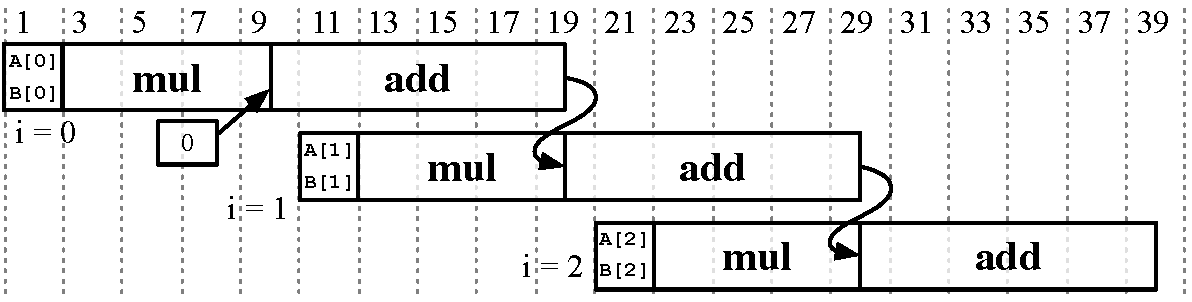
\includegraphics[width=0.8\linewidth]{sample_schedule_before}
    \caption{%
        The resulting schedule of the example program in generated.
    }\label{bg:fig:sample_schedule_before}
\end{figure}

Any valid schedule of this loop must satisfy the constraints imposed by data
dependences.  For instance in our example, it is clear that in a \emph{single}
iteration, in the loop body, multiplication of \verb|A[i]| and \verb|B[i]|
must precede addition of \verb|d| and the multiplied result.  Furthermore, in
the $(i + 1)$-th iteration, access to the variable \verb|d| must wait until
\verb|d| is updated with a new value in the $i$-th iteration, data dependences
therefore also exist on \verb|d| \emph{across} loop iterations.  We call the
former kind of dependences \emph{intra-iteration dependences} and the latter
\emph{inter-iteration dependences}.

Besides data-dependence constraints, the amount of resources available also
affects loop scheduling.  For instance, under our assumption the RAM can only
be read once per cycle, our schedule thus should avoid reading from the same
RAM in the same clock cycle.  We say a schedule is optimal, in the sense that
the overall latency $L = (N - 1) \times \II + D$, is minimized, while none
of the constraints are violated.  However with a much more complex program,
finding the optimal schedule is often an intractable task.  Limits on resource
availability, along with dependence constraints, make scheduling an NP-hard
problem which is difficult to solve optimally and efficiently~\cite{hwang91}.
A heuristic technique known as modulo SDC scheduling~\cite{zhang13, canis14}
is used in LegUp to efficiently attack the scheduling problem, and is further
discussed below.


\subsection{Modulo SDC Scheduling}
\label{bg:sub:modulo_sdc_scheduling}

\subsubsection{Constructing the Data-Dependence Graph}

In the first stage of modulo SDC scheduling, dependence relations are extracted
from the body of this loop.  These dependence relations form a dependence
graph, where vertices are operations, and edges between pairs of vertices
indicate dependence relations.  This dependence graph can subsequently be used
to derive data-dependence constraints.  Figure~\ref{bg:fig:depgraph} shows
the complete dependence graph of the loop in our Figure~\ref{bg:lst:dotprod}
example.
\begin{figure}[ht]
    \centering
    \begin{tikzpicture}
        \node (ai)  at (0,0) {\texttt{A[i]}};
        \node (bi)  [right=of ai, xshift=5mm] {\texttt{B[i]}};
        \node (mul) [below right=of ai, xshift=-5mm, yshift=5mm]
            {$\times$};
        \node (sum) [left=of mul, xshift=-10mm] {\texttt{d}};
        \node (add) [below right=of sum, xshift=-4mm, yshift=5mm] {$+$};
        \draw[->] (ai)  -- node[near start, below=1pt]{1} (mul);
        \draw[->] (bi)  -- node[near start, below=1pt]{1} (mul);
        \draw[->] (mul) -- node[near start, below=1pt]{7} (add);
        \draw[->] (sum) -- node[near start, below=1pt]{0} (add);
        \draw[->,dashed]
            (add) to[out=-135, in=180] node[left=3pt]{10 (1)} (sum);
    \end{tikzpicture}
    \caption{%
        The dependence graph formed by the data dependences in the loop body
        of the dot-product example in Figure~\ref{bg:lst:dotprod}.  The dashed
        edge highlights the inter-iteration dependence.
    }\label{bg:fig:depgraph}
\end{figure}

Intra-iteration dependence edges in the graph are labelled with latency value
in cycles accordingly, signifying that the number of clock cycles that must
elapse between the start of the predecessor and the successor operations.  To
illustrate, the edge between the multiplier ``$\times$'' and adder ``$+$'' has
a value of $7$, because ``$\times$'' takes 7 cycles to generate an output.

Additionally, inter-iteration dependences form cycles in the dependence graph.
For example, in each iteration the initial value of \verb|d| depends on the
final value of \verb|d| from the previous iteration.  In this graph we thus add
an edge from the output of the addition to the variable \verb|d|.  We further
describe that this dependence has a \emph{dependence distance} of $1$, as $1$
iteration must elapse between the start of each pair of value updates and its
corresponding use.  This edge is then further assigned an attribute ``$10
(1)$'' which signifies that the adder has a latency of $10$ cycles, and this
dependence has a distance $1$.

\subsubsection{Finding the Minimum Initiation Interval}

Modulo SDC scheduling owes its efficiency to assuming an initial constant $\II$
and attempting to search for a schedule that satisfies this $\II$.  This search
stops if a valid schedule is found, otherwise $\II$ can be incremented by 1 and
search again until we discover a valid schedule.  To begin with, we can find
a lower bound---which we call the minimum initiation interval $\MII$---on the
initial constant $\II$, such that all schedules with an $\II$ less than $\MII$
violate the dependence and resource constraints.


\subsection{Obstacles in Adoption}
\label{sub:obstacles_in_adoption}


